\documentclass{article}
\usepackage[utf8]{inputenc}
\usepackage{amsmath}
\usepackage{amssymb}
\usepackage{graphicx}
\usepackage{mathtools}

\RenewCommandCopy{\Hat}{\hat}
\usepackage{realhats}

\graphicspath{{Images/}}
\setlength{\oddsidemargin}{0in}
\setlength{\textwidth}{6.5in}
\setlength{\topmargin}{-.55in}
\setlength{\textheight}{9in}
\pagestyle{empty}


\title{Optimization HW 2}
\author{Michael Nameika}
\date{February 2023}

\begin{document}

\maketitle

\section*{Section 2.5 Problems}
\textbf{1.} For each of the following sequences, prove that the sequence cconverges, find its limit, and determine the rate of convergence and the rate constant.
\begin{itemize}
    \item[(i)] The sequence
    \[\frac{1}{2}, \frac{1}{4}, \frac{1}{8}, \frac{1}{16}, \frac{1}{32}, \ldots\]
    with general term $x_k = 2^{-k}$, for $k = 1, 2, \dots$.
    \newline\newline
    I claim $x_k \to x_* =0$.
    \newline
    Proof: Fix $\epsilon > 0$ and let $n > N \in \mathbb{N}$. Then
    \[|x_n - x_*| = \left|\frac{1}{2^n} - 0\right|\]
    Notice
    \begin{align*}
        n &> N \\
        2^n &> 2^N \\
        \frac{1}{2^n} &< \frac{1}{2^N} \\
    \end{align*}
    Choose $N$ such that $\frac{1}{2^N} \leq \epsilon$. That is, choose $N$ such that
    \[N \geq -\log_2(\epsilon)\]
    Then for all $n > N$,
    \begin{align*}
        \left|\frac{1}{2^n} - 0\right| &= |x_n - x_*| < \epsilon \\
    \end{align*}
    So $x_k \to 0$.
    \newline\newline
    To find the rate of convergence and the rate constant, notice
    \begin{align*}
        |e_k| &= |x_k - x_*| = \left|\frac{1}{2^k}\right| \\
        \lim_{k\to \infty} \frac{|e_{k+1}|}{|e_k|} &= \lim_{k \to \infty} \frac{1/2^{k+1}}{1/2^k} \\
        &= \lim_{k \to \infty} \frac{1}{2} \\
        &= \frac{1}{2} \\
    \end{align*}
    So $\{x_k\}$ converges linearly with rate constant $C = 1/2$. 

    \item[(ii)] The sequence 
    \[1.05, 1.0005, 1.000005, \dots\]
    with general term $x_k = 1 + 5 \times 10^{-2k}$, for $k = 1, 2, \dots$.
    \newline\newline
    I claim that $x_k \to x_* = 1$. 
    \newline
    Proof: Fix $\epsilon > 0$ and let $n > N \in \mathbb{N}$ and consider $|x_n - x_*|$:
    \begin{align*}
        |x_n - X_*| &= |1 + 5\times 10^{-2k} -1| \\
        &= |5\times 10^{-2k}| \\
    \end{align*}
    Choose $N$ such that $5\times 10^{-2N} \leq \epsilon$, or alternatively,
    \[N \geq -\frac{1}{2}\log_{10}\left(\frac{\epsilon}{5}\right)\]
    Then
    \begin{align*}
        |1 + 5 \times 10^{-2n} - 1| < \epsilon
    \end{align*}
    so $x_k \to 1$. 
    \newline\newline
    To find the rate of convergence and the rate constant, notice
    \begin{align*}
        |e_k| &= |x_k - x_*| = |1 + 5\times 10^{-2k} - 1| \\
        \lim_{k\to \infty} \frac{|e_{k+1}|}{|e_k|} &= \lim_{k \to \infty} \frac{5\times 10^{-2(k+1)}}{5\times 10^{-2k}} \\
        \lim_{k \to \infty} \frac{1}{100} &= \frac{1}{100} \\
    \end{align*}
    So $\{x_k\}$ converges linearly with rate constant $C = 1/100$.

    \item[(iii)] The sequence with general term $x_k = 2^{-2^k}$.
    \newline\newline
    I claim that $x_k \to x_* = 0$. 
    \newline
    Proof: Fix $\epsilon > 0$ and let $n > N \in \mathbb{N}$ and consider $|x_n - x_*|$:
    \begin{align*}
        |x_n - x_*| &= |2^{-2^n} - 0| \\
        &= 2^{-2^n} \\
    \end{align*}
    Choose $N$ such that $2^{-2^N} \leq \epsilon$. Then 
    \[N \geq -\frac{1}{2}\log_2(\epsilon)\]
    Then we have
    \[|2^{-2^n} - 0| < \epsilon\]
    for all $n > N$. So $x_k \to 0$.
    \newline\newline
    To find the rate of convergence and rate constant, notice
    \begin{align*}
        |e_k| &= |x_k - x_*| = |2^{-2^k}| \\
        \lim_{k \to \infty} \frac{|e_{k+1}|}{|e_k|^2} &= \lim_{k \to \infty} \frac{2^{-2^{k+1}}}{(2^{-2^k})^2} \\
        &= \lim_{k \to \infty} \frac{2^{-2^{k+1}}}{2^{-2^{k+1}}} \\
        &= 1 \\
    \end{align*}
    So $\{x_k\}$ converges quadratically with rate constant $C = 1$.

    \item[(iv)] The sequence with general term $x_k = 3^{-k^2}$.
    \newline\newline
    I claim $x_k \to x_* = 0$.
    \newline
    Proof: Fix $\epsilon > 0$ and let $n > N\in \mathbb{N}$ and consider $|x_k - x_*| = |3^{-k^2} - 0|$. Since $n > N$,
    \begin{align*}
        n^2 &> N^2 \\
        -n^2 &< -N^2 \\
        3^{-n^2} &< 3^{-N^2} \\
    \end{align*}
    Choose $N$ such that $3^{-N^2} \leq \epsilon$. Or alternatively,
    \[N^2 \geq -\log_3(\epsilon)\]
    Then $|3^{-n^2} - 0| < \epsilon$, so $x_k \to 0$.
    \newline\newline
    To find the rate of convergence and rate constant, notice
    \begin{align*}
        |e_k| &= |3^{-k^2}| \\
        \lim_{k\to\infty} \frac{|e_{k+1}|}{|e_k|} &= \lim_{k\to\infty} \frac{3^{-(k+1)^2}}{3^{-k^2}} \\
        &= \lim_{k\to\infty} 3^{-2k-1} = 0 \\
    \end{align*}
    Since $r = 1$ and $C = 0$, we have that $\{x_k\}$ converges superlinearly.

    \item[(v)] The sequence with general term $x_k = 1 - 2^{-2^k}$ for $k$ odd, and $x_k = 1 + 2^{-k}$ for $k$ even.
    \newline\newline
    I claim that $x_k \to x_* = 1$. 
    \newline
    Proof: To prove $\{x_k\}$ converges, we will show that the even and odd subsequences of $\{x_k\}$ converge to the same limit. For $k$ odd, I claim that $x_k \to 1$. In this case, fix $\epsilon > 0$, let $n > N \in \mathbb{N}$ and consider $|1 - 2^{-2^k} - 1| = 2^{-2^k}$. Since $n > N$,
    \begin{align*}
        -2^n &< -2^N \\
        2^{-2^n} &< 2^{-2^N} \\
    \end{align*}
    Choose $N$ such that $2^{-2N} \leq \epsilon$, or equivalently, choose $N$ such that $N \geq -1/2\log_2(\epsilon)$. Then
    \begin{align*}
        |1 - 2^{-2^n} - 1| &< \epsilon \\
    \end{align*}
    for all $n > N$. So the odd terms of $x_k$ converge to 1. Again, fix $\epsilon > 0$ not necessarily the same as $\epsilon$ previously defined, and likewise let $n > N \in \mathbb{N}$ and consider $|1 + 2^{-n} - 1| = 2^{-n}$. Since $n > N$,
    \begin{align*}
        -n &< -N \\
        2^{-n} &< 2^{-N} \\
    \end{align*}
    Choose $N$ such that $2^{-N} \leq \epsilon$, or equivalently, choose $N$ such that $N \geq -\log_2(\epsilon)$. Then
    \[|1 + 2^{-n} - 1| < \epsilon\]
    for all $n > N$. So $\{x_k\} \to 1$ since the odd and even subsequences converge to the same limit.
    \newline\newline
    To find the rate of convergence and rate constant, let us inspect the odd and even subsequences. Let us begin with odd $k$ and notice
    \begin{align*}
        \lim_{k\to\infty}\frac{|e_{k+1}|}{|e_k|^2} &= \lim_{k\to\infty}\frac{2^{-2^{k+1}}}{(2^{-2^k})^2} \\
        &= \lim_{k\to\infty} \frac{2^{-2^{k+1}}}{2^{-2^{k+1}}} \\
        &= 1
    \end{align*}
    So $\{x_k\}$ converges quadratically for $k$ odd. Now let us inspect the even subsequence and notice
    \begin{align*}
        \lim_{k\to\infty} \frac{|e_{k+1}|}{|e_k|} &= \lim_{k\to\infty} \frac{2^{-(k+1)}}{2^{-k}} \\
        &= \frac{1}{2}
    \end{align*}
    So $\{x_k\}$ converges linearly for $k$ even. 

    \end{itemize}

    \section*{Section 2.7 Problems}
    \textbf{1.} Apply Newton's method to find all three solutions of
    \[f(x) = x^3 - 5x^2 - 12x + 19 = 0\]
    You will have to use several different initial guesses.
    \newline\newline
    Implementing Newton's method in a simple MATLAB script, we find the following solutions for $f(x) = 0$:
    \newline
    \begin{center}
        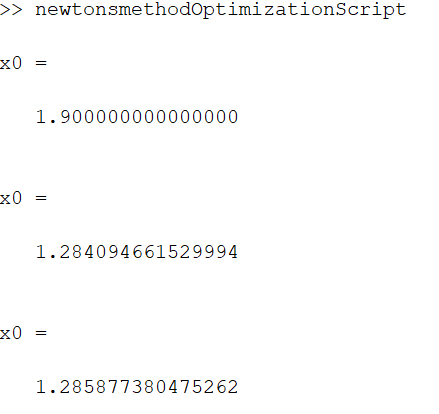
\includegraphics[scale = 0.6]{prob_2_7_1_1}
        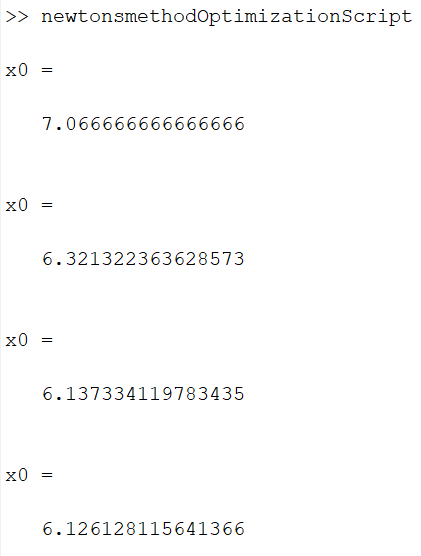
\includegraphics[scale = 0.6]{prob_2_7_1_2}
        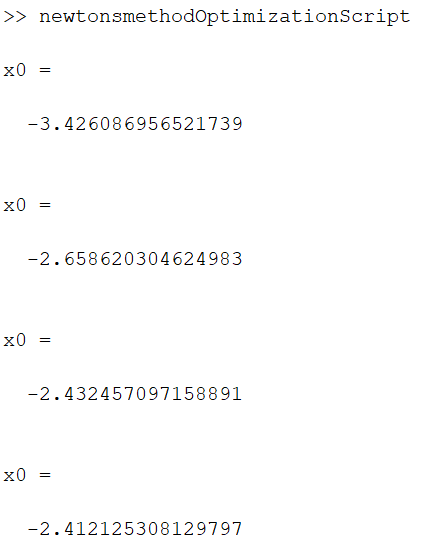
\includegraphics[scale = 0.6]{prob_2_7_1_3}
        \newline
    \end{center}
    The above figures show the outputs for initial guesses of $x_0 = 0,5,-5$ respectively. An error tolerance was chosen to be 1e-2. From this, we can see the solutions to $f(x) = 0$ are approximately $x_1 = 1.286$, $x_2 = 6.126$, $x_3 = -2.412$.
    \newline\newline

    \textbf{5.} Apply Newton's method to solve $f(x) = x^2 - a = 0$, where $a > 0$. Here, choose $a = 2$ and highlight the quadratic convergence.
    \newline\newline
    Modifying the script used for problem 1, using $x_0 = 20$ (to get more iterations to show convergence), we find that $f(x) = 0$ at approximately $x = 1.4142$. The following plot displays that the convergence of the method was roughly quadratic. By inspection, if $a < 0$, any strictly real initial guess will not converge. However, if $x_0 \in \mathbb{C}$, we should expect the method to converge to one of the complex roots. In fact this is what we see for the example using $f(x) = x^2 + 4$ with initial guess $1 + i$.
    \begin{center}
        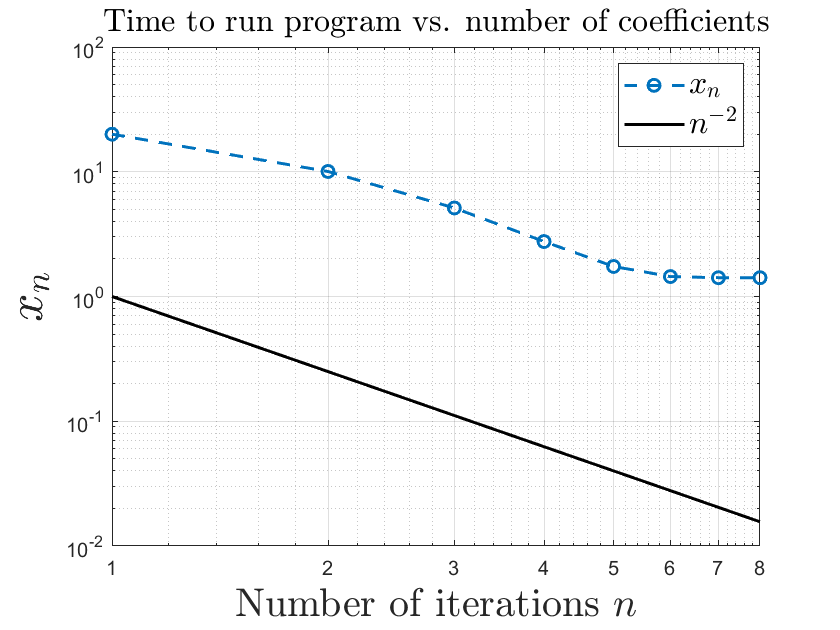
\includegraphics[scale = 0.5]{2_7_5_plot.png}
    \end{center}
    \begin{center}
        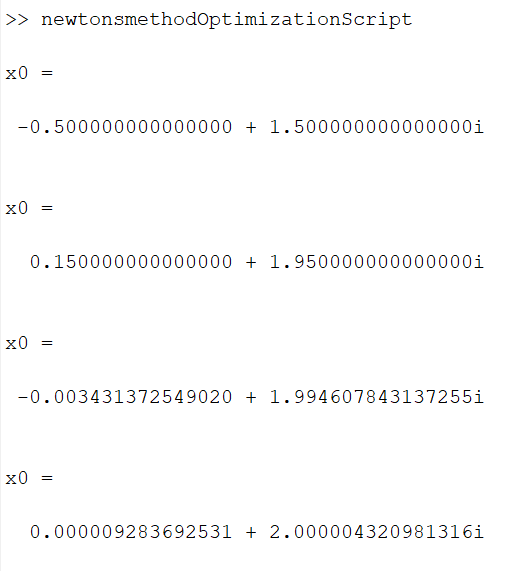
\includegraphics[scale = 0.75]{complex root convergence}
    \end{center}

    \textbf{10.} Apply Newton's method to the system of nonlinear equations
    \begin{align*}
        f_1(x_1,x_2) &= x_1^2 + x_2^2 - 1 = 0\\
        f_2(x_1,x_2) &= 5x_1^2 - x_2 - 2 = 0 \\
    \end{align*}
    There are four solutions to this system of equations. Can you find all four of them by using different initial guesses?
    \newline\newline
    Given $f_1(x)$ and $f_2(x)$, we have
    \[f(x) = \begin{pmatrix}
        x_1^2 + x_2^2 - 1 \\
        5x_1^2 - x_2 - 2 \\
    \end{pmatrix}\]
    and we find the following for the Jacobian of $f$:
    \[\nabla f(x)^T = \begin{pmatrix}
        2x_1 & 2x_2 \\
        10x_1 & -1 \\
    \end{pmatrix}\]
    Implementing Newton's method for higher dimensions into MATLAB, we find the following minima of $f(x)$:
    \begin{align*}
        x_1 &= \begin{pmatrix}
            0.7323\\
            0.6810 \\
        \end{pmatrix}
        \:\: x_2 = \begin{pmatrix}
            -0.4731\\
            -0.8810\\
        \end{pmatrix}\\
        x_3 &= \begin{pmatrix*}[r]
            -0.7323\\
            0.6810\\
        \end{pmatrix*}
        \:\: x_4 = \begin{pmatrix*}[r]
            0.4731\\
            -0.8810\\
        \end{pmatrix*}
    \end{align*}
    using initial guesses $x_{1,0} = (1,1)^T$, $x_{2,0} = (-1,-1)^T$, $x_{3,0} = (-1,1)^T$, and $x_{4,0} = (1,-1)^T$, respectively.


    \section*{Section 3.1 Problems}
    \textbf{2.} Consider the set defined by the constraints $x_1 + x_2 = 1$, $x_1 \geq 0$, and $x_2 \geq 0$. At each of the following points determine the set of feasible directions: (a) $(0,1)^T$; (b) $(1,0)^T$; (c) $(0.5, 0.5)^T$.
    \newline\newline
    From the given constraints above, we have 
    \begin{align*}
        a_1 &= (1,1)^T, \:\:\:\:\: b_1 = 1\\
        a_2 &= (1,0)^T, \:\:\:\:\: b_2 = 0\\
        a_3 &= (0,1)^T, \:\:\:\:\: b_3 = 0\\
    \end{align*}
    \begin{itemize}
        \item[(a)] $\bar{x} = (0,1)^T$. 
        \newline\newline
        Notice that the constraints $a_1, a_3$ are active and $a_2$ is inactive. Then a feasible direction $p$ must satisfy
        \begin{align*}
            a_1^Tp &= 0\\
            a_3^Tp &\geq 0\\
        \end{align*}
        From this, we have
        \begin{align*}
            p_1 &= -p_2 \\
            p_2 &\geq 0\\
        \end{align*}
        So the set of feasible directions at $\bar{x}$ is given by
        \[P = \left\{\begin{pmatrix*}[r]
            -1\\
            1\\
        \end{pmatrix*}t \:\: \bigg| \:\: t \in \mathbb{R}, \: t \geq 0\right\}\]

        \item[(b)] $\bar{x} = (1,0)^T$
        \newline\newline
        Notice that the constraints $a_1$ and $a_2$ are active and the constraint $a_3$ is inactive. Then a feasible direction $p$ must satisfy
        \begin{align*}
            a_1^Tp &= 0\\
            a_2^TP &\geq 0\\
        \end{align*}
        From this, we have
        \begin{align*}
            p_1 &= -p_2 \\
            p_1 &\geq 0\\
        \end{align*}
        So the set of feasible directions at $\bar{x}$ is given by
        \[P = \left\{\begin{pmatrix*}[r]
            -1\\
            1\\
        \end{pmatrix*}t \:\: \bigg| \:\: t \in \mathbb{R}, \: t \leq 0\right\}\]

        \item[(c)] $\bar{x} = (0.5,0.5)^T$.
        \newline\newline
        Notice that the constraint $a_1$ is active and the constraints $a_2$ and $a_3$ are inactive. Then a feasible direction $p$ must satisfy
        \[a_1^Tp = 0\]
        From this, we have
        \[p_1 = -p_2\]
        So the set of feasible direction at $\bar{x}$ is given by
        \[P = \left\{\begin{pmatrix*}[r]
            -1\\
            1\\
        \end{pmatrix*}t \:\: \bigg| \:\: t\in \mathbb{R}\right\}\]
        
        
    \end{itemize}



    \textbf{3.} Consider the system of inequality constraints $Ax \geq b$ with
    \[A = \begin{pmatrix*}[r]
        9 & 4 & 1 & 9 & -7\\
        6 & -7 & 8 & -4 & -6\\
        1 & 6 & 3 & -7 & 6\\
    \end{pmatrix*}
    \:\:\:\: \text{ and } \:\:\:\: b = \begin{pmatrix}
        -15\\
        -30\\
        -20\\
    \end{pmatrix}
    \]
    For the given values of $x$ and $p$, perform a ratio test to determine the maximum step length $\bar{\alpha}$ such that $x + \bar{\alpha}p$ remains feasible.
    \newline\newline
    From the matrix $A$ and vector $b$ above, we have the following constraints:
    \begin{align*}
        a_1 &= (9,4,1,9,-7)^T \:\:\:\:\:\:\:\:\:\:\:\: b_1 = -15\\
        a_2 &= (6,-7,8,-4,-6)^T \:\:\:\:\: b_2 = -30\\
        a_3 &= (1,6,3,-7,6)^T \:\:\:\:\:\:\:\:\:\:\:\: b_3 = -20\\
    \end{align*}
    \begin{itemize}
        \item[(i)] $x = (8,4,-3,4,1)^T$ and $p = (1,1,1,1,1)^T$,
        \newline\newline
        To begin, let us verify the constraints are inactive for $x$:
        \begin{align*}
            a_1^Tx &= 9(8) + 4(4) + 1(-3) + 9(4) + -7(1) = 72 + 16 - 3 + 36 - 7 = 114 > b_1\\
            a_2^Tx &= 6(8) + -7(4) + 8(-3) + -4(4) + -6(1) = 48 - 28 - 24 - 16 - 6 = -26 > b_2\\
            a_3^Tx &= 1(8) + 6(4) + 3(-3) + -7(4) + 6(1) = 8 + 24 - 9 - 28 + 6 = 1 > b_3\\
        \end{align*}
        So all three constraints are inactive for $x$. Now, let us determine which constraints are relevant for finding the upper bound on $\alpha$:
        \begin{align*}
            a_1^Tp &= 9 + 4 + 1 + 9 - 7 = 16\\
            a_2^Tp &= 6 - 7 + 8 - 4 - 6 = -3\\
            a_3^Tp &= 1 + 6 + 3 - 7 + 6 = 9\\
        \end{align*}
        So the only constraint that is relevant is $a_2$. Then
        \begin{align*}
            \bar{\alpha} &= \frac{a_2^Tx - b_2}{-a_2^Tp} \\
            &= \frac{-26 + 30}{3} \\
            &= \frac{4}{3} \\
        \end{align*}
        So we have our upper bound for $\alpha$ is $\bar{\alpha} = 4/3$.
        

        \item[(ii)] $x = (7,-4,-3,-3,3)^T$ and $p = (3,2,0,1,-2)^T$,
        \newline\newline
        As in part (i), let us verify the constraints are inactive for $x$:
        \begin{align*}
            a_1^Tx &= 9(7) + 4(-4) + 1(-3) + 9(-3) + -7(3) = 63 - 16 - 3 - 27 - 21 = -4 > b_1\\
            a_2^Tx &= 6(7) + -7(-4) + 8(-3) + -4(-3) + -6(3) = 42 + 28 - 24 + 12 - 18 = 40 > b_2 \\
            a_3^Tx &= 1(7) + 6(-4) + 3(-3) + -7(-3) + 6(3) = 7 - 24 - 9 + 21 + 18 = 13 > b_3 \\
        \end{align*}
        So all three constraints are inactive for $x$. Now let us determine which constraints are relevant for finding the upper bound on $\alpha$:
        \begin{align*}
            a_1^Tp &= 9(3) + 4(2) + 1(0) + 9(1) + -7(-2) = 27 + 8 + 9 + 14 = 58 \\
            a_2^Tp &= 6(3) + -7(2) + 8(0) + -4(1) + -6(-2) = 18 - 14 - 4 + 12 = 12\\
            a_3^Tp &= 1(3) + 6(2) + 3(0) + -7(1) + 6(-2) = 3 + 12 - 7 - 12 = -4\\
        \end{align*}
        So $a_3$ is the only relevant constraint. Then
        \begin{align*}
            \bar{\alpha} &= \frac{a_3^Tx - b_3}{-a_3^Tp} \\
            &= \frac{13 + 20}{4} \\
            &= \frac{33}{4} \\
        \end{align*}
        So we have our upper bound for $\alpha$ is $\bar{\alpha} = 33/4$.

        \item[(iii)] $x = (5,0,-6,-8,-3)^T$ and $p = (5,0,5,1,3)^T$.
        \newline\newline
        Let us begin by verifying the constraints are inactive for $x$:
        \begin{align*}
            a_1^Tx &= 9(5) + 4(0) + 1(-6) + 9(-8) + -7(-3) = 45 - 6 - 72 + 21 = -12 > b_1 \\
            a_2^Tx &= 6(5) + -7(0) + 8(-6) + -4(-8) + -6(-3) = 30 - 48 + 18 = 0 > b_2 \\
            a_3^Tx &= 1(5) + 6(0) + 3(-6) + -7(-8) + 6(-3) = 5 - 18 + 56 - 18 = 25 > b_3 \\
        \end{align*}
        So all three constraints are inactive for $x$. Now let us determine which constraints are relevant for finding the upper bound on $\alpha$:
        \begin{align*}
            a_1^Tp &= 9(5) + 4(0) + 1(5) + 9(1) + -7(3) = 45 + 5 + 9 - 21 = 38 \\
            a_2^Tp &= 6(5) + -7(0) + 8(5) + -4(1) + -6(3) = 35 + 40 - 4 - 18 = 53 \\
            a_3^Tp &= 1(5) + 6(0) + 3(5) + -7(1) + 6(3) = 5 + 15 - 7 + 18 = 31 \\
        \end{align*}
        Since none of the constraints are relevant, this means that the constraints will remain satisfied for all $\alpha \geq 0$.
        
        \item[(iv)] $x = (9,1,-1,6,3)^T$ and $p = (-4,-2,4,-2,2)^T$.
        \newline\newline
        Let us begin by verifying the constraints are inactive for $x$:
        \begin{align*}
            a_1^Tx &= 9(9) + 4(1) + 1(-1) + 9(6) + -7(3) = 81 + 4 - 1 + 54 - 21 = 117 > b_1\\
            a_2^Tx &= 6(9) + -7(1) + 8(-1) + -4(6) + -6(-3) = 54 - 7 - 8 - 24 + 18 = 33 > b_2\\
            a_3^Tx &= 1(9) + 6(1) + 3(-1) + -7(6) + 6(3) = 9 + 6 - 3 - 42 + 18 = -12 > b_3\\
        \end{align*}
        So all three constraints are inactive for $x$. Now let us determine which constraints are relevant for finding the upper bound on $\alpha$:
        \begin{align*}
            a_1^Tp &= 9(-4) + 4(-2) + 1(4) + 9(-2) + -7(2) = -36 - 8 + 4 - 18 - 14 = -72\\
            a_2^Tp &= 6(-4) + -7(-2) + 8(4) + -4(-2) + -6(2) = -24 + 14 + 32 + 8 - 12 = 18\\
            a_3^Tp &= 1(-4) + 6(-2) + 3(4) + -7(-2) + 6(2) = -4 - 12 + 12 + 14 + 12 = 22\\
        \end{align*}
        So $a_1$ is the only relevant constraint. Then
        \begin{align*}
            \bar{\alpha} &= \frac{a_1^Tx - b_1}{-a_1^Tp}\\
            &= \frac{117 + 15}{72} \\
            &= \frac{132}{72} \\
            &= \frac{33}{18} \\
        \end{align*}
        So we have our upper bound for $\alpha$ is $\bar{\alpha} = 33/18$.
        
    \end{itemize}


    \section*{Section 3.2 Problems}
    \textbf{1.} In each of the following cases, compute a basis matrix for the null space of the matrix $A$ and express the points $x_i$ as $x_i = p_i + q_i$ where $p_i$ is in the null space of $A$ and $q_i$ is in the range space of $A^T$.
    \begin{itemize}
        \item[(i)] 
        \[A = \begin{pmatrix*}[r]
            1 & 1 & 1 & 1\\
            1 & -1 & -1 & 1\\
            0 & 1 & 0 & 1\\
        \end{pmatrix*}, \:\:\:\: x_1 = \begin{pmatrix*}[r]
            1\\
            3\\
            1\\
            2\\
        \end{pmatrix*}, \:\:\:\: x_2 = \begin{pmatrix*}[r]
            0\\
            -2\\
            -3\\
            4\\
        \end{pmatrix*}\]
        Let us begin by finding a basis matrix for the null space of $A$. Recall $p \in \mathcal{N}(A)$ when $Ap = 0$, or
        \[\begin{pmatrix*}[r]
            1 & 1 & 1 & 1\\
            1 & -1 & -1 & 1\\
            0 & 1 & 0 & 1\\
        \end{pmatrix*}\begin{pmatrix*}[r]
            p_1\\
            p_2\\
            p_3\\
            p_4\\
        \end{pmatrix*} = \begin{pmatrix}
            0\\
            0\\
            0\\
            0\\
        \end{pmatrix}\]
        Which gives us the linear system 
        \begin{align*}
            &p_1 + p_2 + p_3 + p_4 = 0 \\
            &p_1 - p_2 + p_3 - p_4 = 0 \\
            &p_2 + p_4 = 0\\
        \end{align*}
        which gives us the following basis matrix for the null space of $A$:
        \[Z = \begin{pmatrix*}[r]
            -1\\
            -1\\
            1\\
            1\\
        \end{pmatrix*}\]
        Now, using this matrix and the rows of $A$, we find the following for $x_1$ and $x_2$:
        \begin{align*}
            x_1 &= \begin{pmatrix*}[r]
                3/4\\
                11/4\\
                5/4\\
                9/4\\
            \end{pmatrix*} + \begin{pmatrix*}[r]
                -13/4\\
                11/4\\
                15/4\\
                -13/4\\
            \end{pmatrix*}\\
        \end{align*}
        Where $(3/4,11/4,5/4,9/4)^T \in R(A^T)$, $(-13/4,11/4,15/4,-13/4)^T \in \mathcal{N}(A)$. And
        \begin{align*}
            x_2 &= \begin{pmatrix*}[r]
                3/4\\
                -5/4\\
                -15/4\\
                13/4\\
            \end{pmatrix*} + \begin{pmatrix*}[r]
                -3/4\\
                -3/4\\
                3/4\\
                3/4\\
            \end{pmatrix*}\\
        \end{align*}    
        Where $(3/4, -5/4, -15/4, 13/4)^T \in R(A^T)$, $(-3/4,-3/4,3/4,3/4)^T \in \mathcal{N}(A)$.
        
        \item[(ii)]
        \[A = \begin{pmatrix*}[r] 
            1 & 1 & 1 & 1\\
        \end{pmatrix*}, \:\:\:\: x_1 = \begin{pmatrix*}[r]
            -2\\
            4\\
            5\\
            -2\\
        \end{pmatrix*}, \:\:\:\: x_2 = \begin{pmatrix*}[r]
            7\\
            5\\
            -13\\
            1\\
        \end{pmatrix*}\]
        To begin, let us determine a basis matrix for the null space of $A$:
        \begin{align*}
            \begin{pmatrix*}[r]
                1 & 1 & 1 & 1\\
            \end{pmatrix*}\begin{pmatrix*}[r]
                p_1\\
                p_2\\
                p_3\\
                p_4\\
            \end{pmatrix*} &= \begin{pmatrix}
                0\\
                0\\
                0\\
                0\\
            \end{pmatrix}\\
        \end{align*}
        Which gives us the linear equation $p_1 + p_2 + p_3 + p_4 = 0$, which corresponds to a basis matrix for the null space of 
        \[Z = \begin{pmatrix*}[r]
            -1 & -1 & -1\\
            1 & 0 & 0\\
            0 & 1 & 0\\
            0 & 0 & 1\\
        \end{pmatrix*}\]
        Using the matrix $Z$ and the row of $A$, we find the following for $x_1$ and $x_2$:
        \begin{align*}
            x_1 &= \begin{pmatrix*}[r]
                5/4\\
                5/4\\
                5/4\\
                5/4\\
            \end{pmatrix*} + \begin{pmatrix*}[r]
                -13/4\\
                11/4\\
                15/4\\
                -13/4\\
            \end{pmatrix*}
        \end{align*}
        where $(5/4, 5/4, 5/4, 5/4)^T \in R(A^T)$, $(-13/4,11/4,15/4,-13/4)^T \in \mathcal{N}(A)$. Notice that $Ax_2 = 0$, so $x_2 \in \mathcal{N}(A)$, so $x_2$ is already written as a sum of vectors from the row space and null space of $A$.
    \end{itemize}

    \textbf{2.} Let $Z$ be an $n \times r$ null-space matrix for the matrix $A$. If $Y$ is any invertible $r \times r$ matrix, prove that $\Hat{Z} = ZY$ is also a null-space matrix for $A$.
    \newline\newline
    Proof: Let $Z$ be a null space matrix for $A$ and let $Y$ be an invertible $r \times r$ matrix and let $v \in \mathbb{R}^r$ and consider $Yv$:
    \[Yv = \Hat{v}\]
    And notice that $Z\Hat{v}$ gives us a linear combination of the rows of $Z$, which means that $Z\Hat{v}$ is in the null space of $A$. That is, $ZY$ is also a null space matrix for $A$.
\newline\newline

    \textbf{3.} Let $A$ be a given $m \times n$ matrix and let $Z$ be a null-space matrix for $A$. Let $X$ be an invertible $m \times m$ matrix and let $Y$ be an invertible $n \times n$ matrix. If a change of variable is made to transform $A$ into $\Hat{A} = XAY$, how can $Z$ be transformed into $\Hat{Z}$, a null-space matrix for $\Hat{A}$?
    \newline\newline
    We can transform $Z$ into $\Hat{Z}$, a null-space matrix for $\hat[tophat]{A}$ by observing the following:
    \begin{align*}
        A &= X^{-1}\hat[tophat]{A}Y^{-1} \\
    \end{align*}
    Suppose $p \in N(A)$, then $p = Zy$ for some $y \in \mathbb{R}^r$. Then we have the following:
    \begin{align*}
        Ap &= 0 \\
        X^{-1}\hat[tophat]{A}Y^{-1}Zy &= 0\\
        \hat[tophat]{A}Y^{-1}Zy &= 0 
    \end{align*}
    Notice then that $Y^{-1}Z$ is a null-space matrix for $\hat[tophat]{A}$, so our transformation is simply
    \[\Hat{Z} = Y^{-1}Z\]

    
\end{document}
